\chapter{Диаграммы прецедентов}
    В данном разделе будут представлены взаимодействия основных пользователей %
    и ролей в системе в виде диаграмм прецедентов и схем активности. Для создания %
    изображений диаграмм было использовано бесплатное программное обеспечения под названием %
    "diagrams.net".\ \cite{diagrams_dot_net} %
    
    \section{Диаграмма прецедентов для сущности "Пользователь"\ }
        Сущность "Пациент"\ имеет следующие возможности:
        \begin{enumerate}
            \item Добавить прием лекарства: Эта возможность позволяет пациенту добавить %
            информацию о приеме лекарства. В процессе добавления создается уведомление, %
            которое отправляется пациенту телеграмм-ботом в определенное время, заданное пациентом;
            \item Добавить визит врача: Эта возможность позволяет пациенту добавить информацию о %
            визите к врачу. В процессе добавления создается уведомление, которое отправляется пациенту %
            телеграмм-ботом в определенное время, заданное пациентом;
            \item Регистрация пациента: Эта возможность позволяет пациенту зарегистрироваться в системе. %
            В процессе регистрации создается экземпляр пациента в базе данных;
            \item Редактирование профиля: Эта возможность позволяет пациенту редактировать свои данные в %
            профиле. В процессе редактирования обновляются данные в базе данных;
            \item Отправка обратной связи: Эта возможность позволяет пациенту отправить обратную связь о системе %
            или услугах. В процессе отправки обновляются данные в базе данных;
        \end{enumerate}
        
        Таким образом, сущность "Пациент"\ имеет пять возможностей, некоторые из которых %
        включают в себя создание уведомления и их отправку телеграмм-ботом, а также обновление %
        данных в базе данных. Диаграмма сущностей изображена на рисунке \ref{patient_uml}.

        \begin{figure}[H]%current location
            \centering
            \scalebox{0.75}{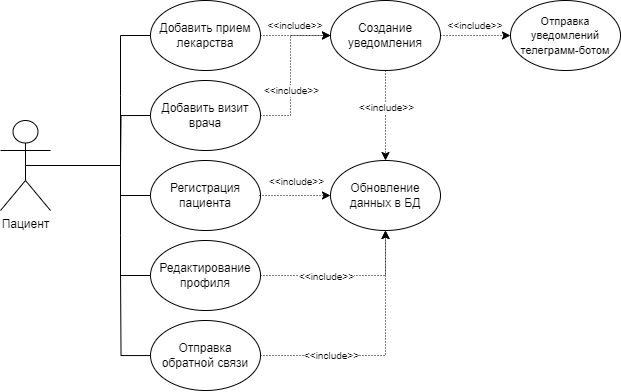
\includegraphics{pics/UML/Patient.png}}
            \caption{Диаграмма прецедентов для роли "Пациент".} \label{patient_uml}
        \end{figure} 
    
    \section{Диаграмма прецедентов для сущности "Доктор"\ }
        Сущность "Доктор"\ имеет следующие возможности:
        \begin{enumerate}
            \item Добавить график лечения пациентов: Эта возможность %
            позволяет доктору добавлять информацию о приемах лекарств %
            для пациента. В процессе добавления создается уведомление, %
            которое отправляется пациенту телеграмм-ботом в определенное %
            время, заданное доктором;
            \item Назначить прием: Эта возможность позволяет доктору %
            назначить прием с пациентом. В процессе добавления создается %
            уведомление, которое отправляется пациенту телеграмм-ботом в %
            определенное время, заданное доктором;
            \item Регистрация доктора: Эта возможность позволяет доктору %
            отправить заявку на регистрацию модератору веб-приложения. %
            В процессе регистрации создается экземпляр доктора с %
            атрибутом, показывающий, что доктор не прошел авторизацию %
            и не подал заявку на подтверждение данных %
            для модератора в базе данных;
            \item Редактирование профиля: Эта возможность позволяет доктору %
            редактировать свои данные в профиле. В процессе редактирования %
            обновляются данные в базе данных;
            \item Получить список пациентов: Эта возможность позволяет доктору %
            получить список лечащихся и уже прошедших лечение пациентов;
        \end{enumerate}
        
        Итоговая диаграмма прецедентов изображена на рисунке \ref{doctor_uml}.

        \begin{figure}[H]%current location
            \centering
            \scalebox{0.70}{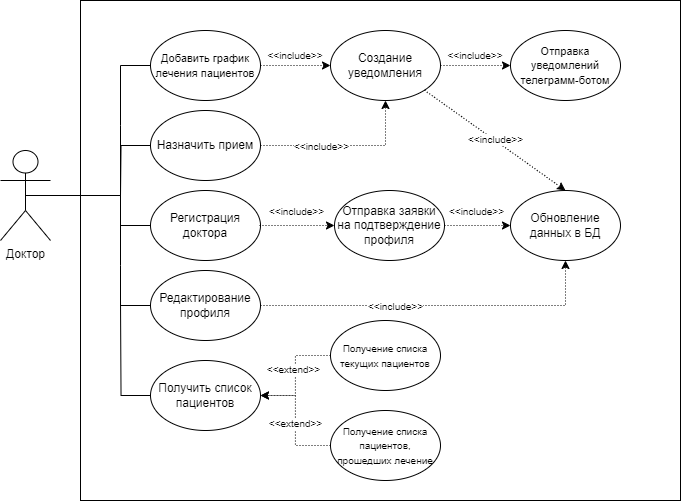
\includegraphics{pics/UML/Doctor.png}}
            \caption{Диаграмма прецедентов для роли "Доктор".} \label{doctor_uml}
        \end{figure} 
    
    \section{Диаграмма прецедентов для сущности "Менеджер"\ }
        Сущность "Менеджер”\ имеет следующие возможности:

        \begin{enumerate}
            \item Получение отзывов о врачах: Эта возможность позволяет менеджеру %
            просмотреть статистику доктора, такую как количество принятых пациентов, %
            проведенных консультаций, выписанных рецептов и других показателей, которые %
            могут помочь оценить эффективность работы доктора. Менеджер может использовать %
            эту информацию для анализа производительности доктора, определения его сильных и %
            слабых сторон, а также для принятия решений о его дальнейшем развитии и обучении. %
            Эта функция также может быть полезна для определения потребностей пациентов и %
            улучшения качества медицинских услуг, предоставляемых клиникой;
            \item Администрирование данных о врачах: Эта возможность позволяет %
             менеджеру подтверждать, отклонять заявку о регистрации доктора, %
             а также, при необходимости, отстранять доктора от врачебной деятельности. %
             Все это влечет за собой обновление данных в БД;
            \item Изменение данных пользователя. Это возможность позволяет менеджеру %
            редактировать данные пациента, которые были указаны при регистрации. %
            При изменении данных пользователя, система автоматически сохраняет новые %
            значения в базе данных, чтобы они были доступны для системных процессов, %
            которые могут нуждаться в этой информации;
        \end{enumerate}
    
        Итоговая диаграмма прецедентов изображена на рисунке \ref{manager_uml}.

        \begin{figure}[H]%current location
            \centering
            \scalebox{0.70}{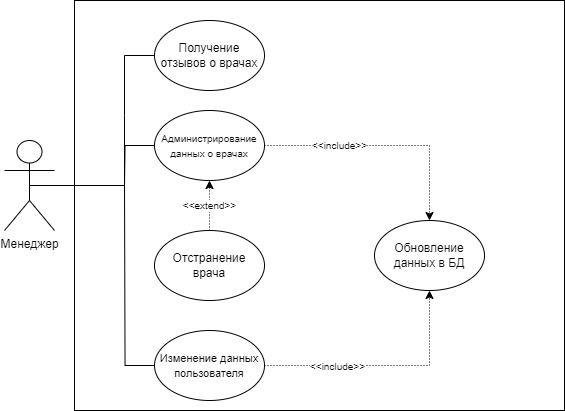
\includegraphics{pics/UML/Manager.png}}
            \caption{Диаграмма прецедентов для роли "Менеджер".} \label{manager_uml}
        \end{figure} 